\item \begin{theorem}{(320)} \quad\quad
    \begin{figure}[H]
        \centering
        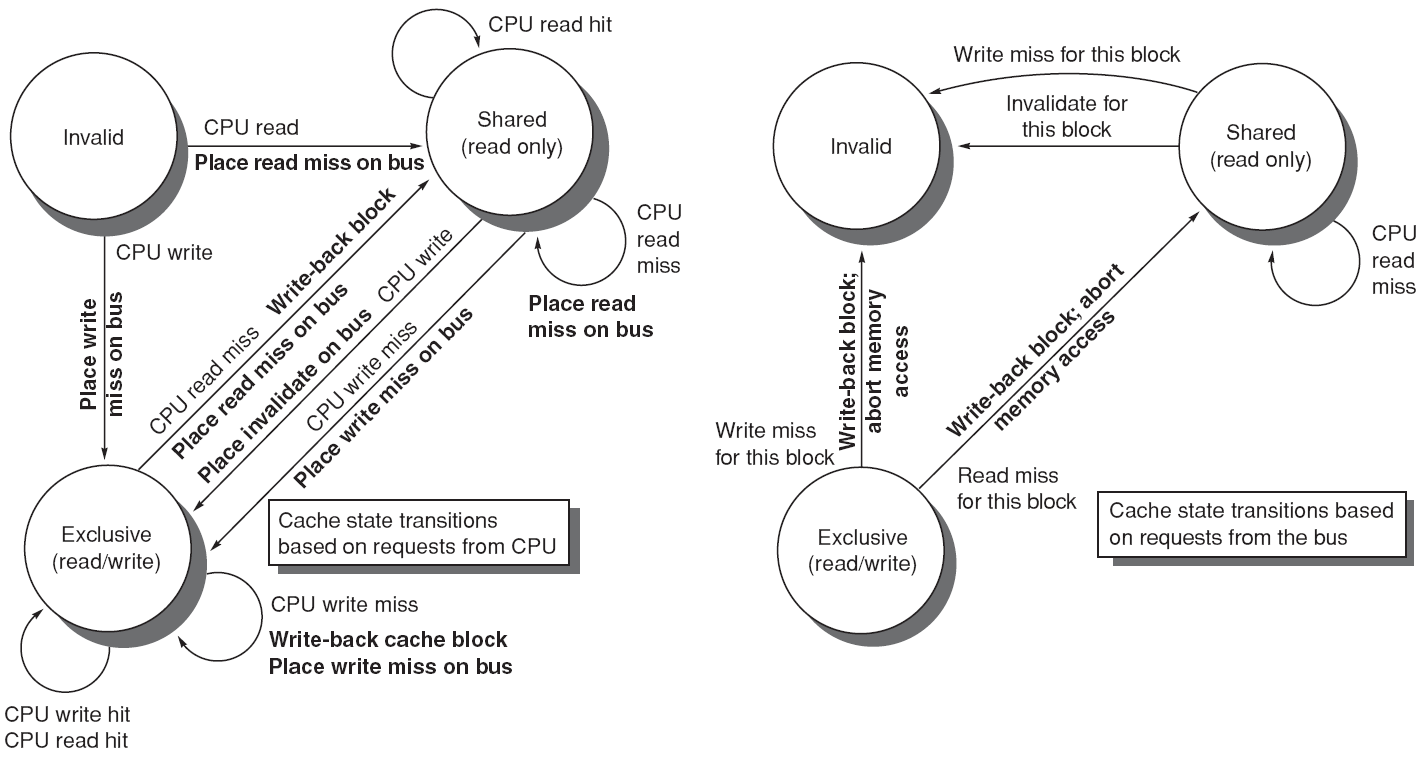
\includegraphics[scale=0.5]{img/snooping.png}
        \caption{Snooping states.}
        \label{img:snooping}
    \end{figure}
\end{theorem}

\item \begin{theorem}{(325)} Multithreading: \begin{itemize}
        \item Coarse-grained multithreading: Switch threads only on costly stalls, such as L2 cache misses. Pipeline \textbf{start-up} costs.
        \item Fine-grained multithreading: Switch between threads on each instruction packs. It can hide the throughput losses.
        \item SMT: \textbf{ILP} and \textbf{TLP}; coarse-grained and fine-grained: \textbf{TLP only}.
    \end{itemize}
\end{theorem}

\item \begin{theorem}{(334)} Network topology: \begin{itemize}
        \item Performance measure:\begin{itemize}
            \item Network bandwidth.
            \item Bisection bandwidth:平均切為二所減少的bandwidth,越高容錯力越高。
            \item Diameter:任兩點最短路的最大值,越低越好。
            \item Nodal degree:CPU degree,越高容錯力越高。
        \end{itemize}
        \item Omega network hardware: $2n\log_2 n$.
        \item Crossbar network hardware: $n^2$.
    \end{itemize}
\end{theorem}
